% Created by tikzDevice version 0.12.3 on 2019-09-26 18:31:02
% !TEX encoding = UTF-8 Unicode
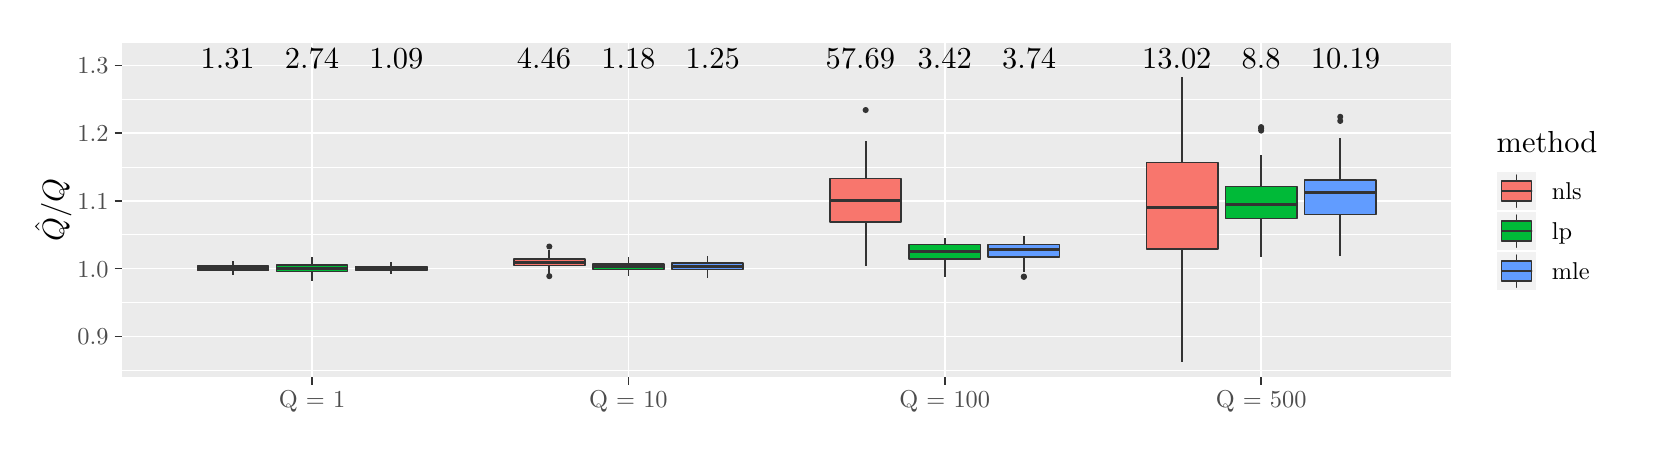
\begin{tikzpicture}[x=1pt,y=1pt]
\definecolor{fillColor}{RGB}{255,255,255}
\path[use as bounding box,fill=fillColor,fill opacity=0.00] (0,0) rectangle (578.16,144.54);
\begin{scope}
\path[clip] (  0.00,  0.00) rectangle (578.16,144.54);
\definecolor{drawColor}{RGB}{255,255,255}
\definecolor{fillColor}{RGB}{255,255,255}

\path[draw=drawColor,line width= 0.6pt,line join=round,line cap=round,fill=fillColor] (  0.00,  0.00) rectangle (578.16,144.54);
\end{scope}
\begin{scope}
\path[clip] ( 34.16, 18.22) rectangle (514.31,139.04);
\definecolor{fillColor}{gray}{0.92}

\path[fill=fillColor] ( 34.16, 18.22) rectangle (514.31,139.04);
\definecolor{drawColor}{RGB}{255,255,255}

\path[draw=drawColor,line width= 0.3pt,line join=round] ( 34.16, 20.74) --
	(514.31, 20.74);

\path[draw=drawColor,line width= 0.3pt,line join=round] ( 34.16, 45.22) --
	(514.31, 45.22);

\path[draw=drawColor,line width= 0.3pt,line join=round] ( 34.16, 69.70) --
	(514.31, 69.70);

\path[draw=drawColor,line width= 0.3pt,line join=round] ( 34.16, 94.19) --
	(514.31, 94.19);

\path[draw=drawColor,line width= 0.3pt,line join=round] ( 34.16,118.67) --
	(514.31,118.67);

\path[draw=drawColor,line width= 0.6pt,line join=round] ( 34.16, 32.98) --
	(514.31, 32.98);

\path[draw=drawColor,line width= 0.6pt,line join=round] ( 34.16, 57.46) --
	(514.31, 57.46);

\path[draw=drawColor,line width= 0.6pt,line join=round] ( 34.16, 81.94) --
	(514.31, 81.94);

\path[draw=drawColor,line width= 0.6pt,line join=round] ( 34.16,106.43) --
	(514.31,106.43);

\path[draw=drawColor,line width= 0.6pt,line join=round] ( 34.16,130.91) --
	(514.31,130.91);

\path[draw=drawColor,line width= 0.6pt,line join=round] (102.75, 18.22) --
	(102.75,139.04);

\path[draw=drawColor,line width= 0.6pt,line join=round] (217.07, 18.22) --
	(217.07,139.04);

\path[draw=drawColor,line width= 0.6pt,line join=round] (331.39, 18.22) --
	(331.39,139.04);

\path[draw=drawColor,line width= 0.6pt,line join=round] (445.71, 18.22) --
	(445.71,139.04);
\definecolor{drawColor}{gray}{0.20}

\path[draw=drawColor,line width= 0.6pt,line join=round] ( 74.17, 58.44) -- ( 74.17, 60.33);

\path[draw=drawColor,line width= 0.6pt,line join=round] ( 74.17, 56.78) -- ( 74.17, 55.20);
\definecolor{fillColor}{RGB}{248,118,109}

\path[draw=drawColor,line width= 0.6pt,line join=round,line cap=round,fill=fillColor] ( 61.31, 58.44) --
	( 61.31, 56.78) --
	( 87.03, 56.78) --
	( 87.03, 58.44) --
	( 61.31, 58.44) --
	cycle;

\path[draw=drawColor,line width= 1.1pt,line join=round] ( 61.31, 57.53) -- ( 87.03, 57.53);

\path[draw=drawColor,line width= 0.6pt,line join=round] (102.75, 58.88) -- (102.75, 61.67);

\path[draw=drawColor,line width= 0.6pt,line join=round] (102.75, 56.48) -- (102.75, 53.14);
\definecolor{fillColor}{RGB}{0,186,56}

\path[draw=drawColor,line width= 0.6pt,line join=round,line cap=round,fill=fillColor] ( 89.89, 58.88) --
	( 89.89, 56.48) --
	(115.61, 56.48) --
	(115.61, 58.88) --
	( 89.89, 58.88) --
	cycle;

\path[draw=drawColor,line width= 1.1pt,line join=round] ( 89.89, 57.60) -- (115.61, 57.60);

\path[draw=drawColor,line width= 0.6pt,line join=round] (131.33, 58.23) -- (131.33, 59.71);

\path[draw=drawColor,line width= 0.6pt,line join=round] (131.33, 56.82) -- (131.33, 55.46);
\definecolor{fillColor}{RGB}{97,156,255}

\path[draw=drawColor,line width= 0.6pt,line join=round,line cap=round,fill=fillColor] (118.47, 58.23) --
	(118.47, 56.82) --
	(144.19, 56.82) --
	(144.19, 58.23) --
	(118.47, 58.23) --
	cycle;

\path[draw=drawColor,line width= 1.1pt,line join=round] (118.47, 57.67) -- (144.19, 57.67);
\definecolor{fillColor}{gray}{0.20}

\path[draw=drawColor,line width= 0.4pt,line join=round,line cap=round,fill=fillColor] (188.49, 54.75) circle (  0.89);

\path[draw=drawColor,line width= 0.4pt,line join=round,line cap=round,fill=fillColor] (188.49, 65.46) circle (  0.89);

\path[draw=drawColor,line width= 0.6pt,line join=round] (188.49, 60.93) -- (188.49, 64.38);

\path[draw=drawColor,line width= 0.6pt,line join=round] (188.49, 58.58) -- (188.49, 55.34);
\definecolor{fillColor}{RGB}{248,118,109}

\path[draw=drawColor,line width= 0.6pt,line join=round,line cap=round,fill=fillColor] (175.63, 60.93) --
	(175.63, 58.58) --
	(201.35, 58.58) --
	(201.35, 60.93) --
	(175.63, 60.93) --
	cycle;

\path[draw=drawColor,line width= 1.1pt,line join=round] (175.63, 59.80) -- (201.35, 59.80);

\path[draw=drawColor,line width= 0.6pt,line join=round] (217.07, 59.18) -- (217.07, 61.65);

\path[draw=drawColor,line width= 0.6pt,line join=round] (217.07, 57.15) -- (217.07, 54.66);
\definecolor{fillColor}{RGB}{0,186,56}

\path[draw=drawColor,line width= 0.6pt,line join=round,line cap=round,fill=fillColor] (204.21, 59.18) --
	(204.21, 57.15) --
	(229.93, 57.15) --
	(229.93, 59.18) --
	(204.21, 59.18) --
	cycle;

\path[draw=drawColor,line width= 1.1pt,line join=round] (204.21, 58.23) -- (229.93, 58.23);

\path[draw=drawColor,line width= 0.6pt,line join=round] (245.65, 59.39) -- (245.65, 62.05);

\path[draw=drawColor,line width= 0.6pt,line join=round] (245.65, 57.16) -- (245.65, 54.24);
\definecolor{fillColor}{RGB}{97,156,255}

\path[draw=drawColor,line width= 0.6pt,line join=round,line cap=round,fill=fillColor] (232.79, 59.39) --
	(232.79, 57.16) --
	(258.51, 57.16) --
	(258.51, 59.39) --
	(232.79, 59.39) --
	cycle;

\path[draw=drawColor,line width= 1.1pt,line join=round] (232.79, 58.20) -- (258.51, 58.20);
\definecolor{fillColor}{gray}{0.20}

\path[draw=drawColor,line width= 0.4pt,line join=round,line cap=round,fill=fillColor] (302.81,114.78) circle (  0.89);

\path[draw=drawColor,line width= 0.6pt,line join=round] (302.81, 90.09) -- (302.81,103.70);

\path[draw=drawColor,line width= 0.6pt,line join=round] (302.81, 74.26) -- (302.81, 58.56);
\definecolor{fillColor}{RGB}{248,118,109}

\path[draw=drawColor,line width= 0.6pt,line join=round,line cap=round,fill=fillColor] (289.95, 90.09) --
	(289.95, 74.26) --
	(315.67, 74.26) --
	(315.67, 90.09) --
	(289.95, 90.09) --
	cycle;

\path[draw=drawColor,line width= 1.1pt,line join=round] (289.95, 82.16) -- (315.67, 82.16);

\path[draw=drawColor,line width= 0.6pt,line join=round] (331.39, 66.20) -- (331.39, 68.49);

\path[draw=drawColor,line width= 0.6pt,line join=round] (331.39, 60.85) -- (331.39, 54.36);
\definecolor{fillColor}{RGB}{0,186,56}

\path[draw=drawColor,line width= 0.6pt,line join=round,line cap=round,fill=fillColor] (318.53, 66.20) --
	(318.53, 60.85) --
	(344.25, 60.85) --
	(344.25, 66.20) --
	(318.53, 66.20) --
	cycle;

\path[draw=drawColor,line width= 1.1pt,line join=round] (318.53, 63.69) -- (344.25, 63.69);
\definecolor{fillColor}{gray}{0.20}

\path[draw=drawColor,line width= 0.4pt,line join=round,line cap=round,fill=fillColor] (359.97, 54.51) circle (  0.89);

\path[draw=drawColor,line width= 0.4pt,line join=round,line cap=round,fill=fillColor] (359.97, 54.60) circle (  0.89);

\path[draw=drawColor,line width= 0.6pt,line join=round] (359.97, 66.19) -- (359.97, 69.44);

\path[draw=drawColor,line width= 0.6pt,line join=round] (359.97, 61.77) -- (359.97, 56.24);
\definecolor{fillColor}{RGB}{97,156,255}

\path[draw=drawColor,line width= 0.6pt,line join=round,line cap=round,fill=fillColor] (347.11, 66.19) --
	(347.11, 61.77) --
	(372.83, 61.77) --
	(372.83, 66.19) --
	(347.11, 66.19) --
	cycle;

\path[draw=drawColor,line width= 1.1pt,line join=round] (347.11, 64.44) -- (372.83, 64.44);

\path[draw=drawColor,line width= 0.6pt,line join=round] (417.13, 95.80) -- (417.13,126.63);

\path[draw=drawColor,line width= 0.6pt,line join=round] (417.13, 64.67) -- (417.13, 23.71);
\definecolor{fillColor}{RGB}{248,118,109}

\path[draw=drawColor,line width= 0.6pt,line join=round,line cap=round,fill=fillColor] (404.27, 95.80) --
	(404.27, 64.67) --
	(430.00, 64.67) --
	(430.00, 95.80) --
	(404.27, 95.80) --
	cycle;

\path[draw=drawColor,line width= 1.1pt,line join=round] (404.27, 79.55) -- (430.00, 79.55);
\definecolor{fillColor}{gray}{0.20}

\path[draw=drawColor,line width= 0.4pt,line join=round,line cap=round,fill=fillColor] (445.71,107.35) circle (  0.89);

\path[draw=drawColor,line width= 0.4pt,line join=round,line cap=round,fill=fillColor] (445.71,108.08) circle (  0.89);

\path[draw=drawColor,line width= 0.4pt,line join=round,line cap=round,fill=fillColor] (445.71,108.60) circle (  0.89);

\path[draw=drawColor,line width= 0.6pt,line join=round] (445.71, 87.12) -- (445.71, 98.58);

\path[draw=drawColor,line width= 0.6pt,line join=round] (445.71, 75.61) -- (445.71, 61.53);
\definecolor{fillColor}{RGB}{0,186,56}

\path[draw=drawColor,line width= 0.6pt,line join=round,line cap=round,fill=fillColor] (432.85, 87.12) --
	(432.85, 75.61) --
	(458.58, 75.61) --
	(458.58, 87.12) --
	(432.85, 87.12) --
	cycle;

\path[draw=drawColor,line width= 1.1pt,line join=round] (432.85, 80.69) -- (458.58, 80.69);
\definecolor{fillColor}{gray}{0.20}

\path[draw=drawColor,line width= 0.4pt,line join=round,line cap=round,fill=fillColor] (474.29,110.85) circle (  0.89);

\path[draw=drawColor,line width= 0.4pt,line join=round,line cap=round,fill=fillColor] (474.29,112.33) circle (  0.89);

\path[draw=drawColor,line width= 0.6pt,line join=round] (474.29, 89.47) -- (474.29,104.64);

\path[draw=drawColor,line width= 0.6pt,line join=round] (474.29, 77.04) -- (474.29, 62.13);
\definecolor{fillColor}{RGB}{97,156,255}

\path[draw=drawColor,line width= 0.6pt,line join=round,line cap=round,fill=fillColor] (461.43, 89.47) --
	(461.43, 77.04) --
	(487.16, 77.04) --
	(487.16, 89.47) --
	(461.43, 89.47) --
	cycle;

\path[draw=drawColor,line width= 1.1pt,line join=round] (461.43, 85.09) -- (487.16, 85.09);
\definecolor{drawColor}{RGB}{0,0,0}

\node[text=drawColor,anchor=base,inner sep=0pt, outer sep=0pt, scale=  1.10] at (133.23,129.75) {1.09};

\node[text=drawColor,anchor=base,inner sep=0pt, outer sep=0pt, scale=  1.10] at (102.75,129.75) {2.74};

\node[text=drawColor,anchor=base,inner sep=0pt, outer sep=0pt, scale=  1.10] at ( 72.26,129.75) {1.31};

\node[text=drawColor,anchor=base,inner sep=0pt, outer sep=0pt, scale=  1.10] at (247.56,129.75) {1.25};

\node[text=drawColor,anchor=base,inner sep=0pt, outer sep=0pt, scale=  1.10] at (217.07,129.75) {1.18};

\node[text=drawColor,anchor=base,inner sep=0pt, outer sep=0pt, scale=  1.10] at (186.59,129.75) {4.46};

\node[text=drawColor,anchor=base,inner sep=0pt, outer sep=0pt, scale=  1.10] at (361.88,129.75) {3.74};

\node[text=drawColor,anchor=base,inner sep=0pt, outer sep=0pt, scale=  1.10] at (331.39,129.75) {3.42};

\node[text=drawColor,anchor=base,inner sep=0pt, outer sep=0pt, scale=  1.10] at (300.91,129.75) {57.69};

\node[text=drawColor,anchor=base,inner sep=0pt, outer sep=0pt, scale=  1.10] at (476.20,129.75) {10.19};

\node[text=drawColor,anchor=base,inner sep=0pt, outer sep=0pt, scale=  1.10] at (445.71,129.75) {8.8};

\node[text=drawColor,anchor=base,inner sep=0pt, outer sep=0pt, scale=  1.10] at (415.23,129.75) {13.02};
\end{scope}
\begin{scope}
\path[clip] (  0.00,  0.00) rectangle (578.16,144.54);
\definecolor{drawColor}{gray}{0.30}

\node[text=drawColor,anchor=base east,inner sep=0pt, outer sep=0pt, scale=  0.88] at ( 29.21, 29.95) {0.9};

\node[text=drawColor,anchor=base east,inner sep=0pt, outer sep=0pt, scale=  0.88] at ( 29.21, 54.43) {1.0};

\node[text=drawColor,anchor=base east,inner sep=0pt, outer sep=0pt, scale=  0.88] at ( 29.21, 78.91) {1.1};

\node[text=drawColor,anchor=base east,inner sep=0pt, outer sep=0pt, scale=  0.88] at ( 29.21,103.40) {1.2};

\node[text=drawColor,anchor=base east,inner sep=0pt, outer sep=0pt, scale=  0.88] at ( 29.21,127.88) {1.3};
\end{scope}
\begin{scope}
\path[clip] (  0.00,  0.00) rectangle (578.16,144.54);
\definecolor{drawColor}{gray}{0.20}

\path[draw=drawColor,line width= 0.6pt,line join=round] ( 31.41, 32.98) --
	( 34.16, 32.98);

\path[draw=drawColor,line width= 0.6pt,line join=round] ( 31.41, 57.46) --
	( 34.16, 57.46);

\path[draw=drawColor,line width= 0.6pt,line join=round] ( 31.41, 81.94) --
	( 34.16, 81.94);

\path[draw=drawColor,line width= 0.6pt,line join=round] ( 31.41,106.43) --
	( 34.16,106.43);

\path[draw=drawColor,line width= 0.6pt,line join=round] ( 31.41,130.91) --
	( 34.16,130.91);
\end{scope}
\begin{scope}
\path[clip] (  0.00,  0.00) rectangle (578.16,144.54);
\definecolor{drawColor}{gray}{0.20}

\path[draw=drawColor,line width= 0.6pt,line join=round] (102.75, 15.47) --
	(102.75, 18.22);

\path[draw=drawColor,line width= 0.6pt,line join=round] (217.07, 15.47) --
	(217.07, 18.22);

\path[draw=drawColor,line width= 0.6pt,line join=round] (331.39, 15.47) --
	(331.39, 18.22);

\path[draw=drawColor,line width= 0.6pt,line join=round] (445.71, 15.47) --
	(445.71, 18.22);
\end{scope}
\begin{scope}
\path[clip] (  0.00,  0.00) rectangle (578.16,144.54);
\definecolor{drawColor}{gray}{0.30}

\node[text=drawColor,anchor=base,inner sep=0pt, outer sep=0pt, scale=  0.88] at (102.75,  7.21) {Q = 1};

\node[text=drawColor,anchor=base,inner sep=0pt, outer sep=0pt, scale=  0.88] at (217.07,  7.21) {Q = 10};

\node[text=drawColor,anchor=base,inner sep=0pt, outer sep=0pt, scale=  0.88] at (331.39,  7.21) {Q = 100};

\node[text=drawColor,anchor=base,inner sep=0pt, outer sep=0pt, scale=  0.88] at (445.71,  7.21) {Q = 500};
\end{scope}
\begin{scope}
\path[clip] (  0.00,  0.00) rectangle (578.16,144.54);
\definecolor{drawColor}{RGB}{0,0,0}

\node[text=drawColor,rotate= 90.00,anchor=base,inner sep=0pt, outer sep=0pt, scale=  1.10] at ( 13.08, 78.63) {$\hat{Q}/Q$};
\end{scope}
\begin{scope}
\path[clip] (  0.00,  0.00) rectangle (578.16,144.54);
\definecolor{fillColor}{RGB}{255,255,255}

\path[fill=fillColor] (525.31, 43.84) rectangle (572.66,113.42);
\end{scope}
\begin{scope}
\path[clip] (  0.00,  0.00) rectangle (578.16,144.54);
\definecolor{drawColor}{RGB}{0,0,0}

\node[text=drawColor,anchor=base west,inner sep=0pt, outer sep=0pt, scale=  1.10] at (530.81, 99.27) {method};
\end{scope}
\begin{scope}
\path[clip] (  0.00,  0.00) rectangle (578.16,144.54);
\definecolor{drawColor}{RGB}{255,255,255}
\definecolor{fillColor}{gray}{0.95}

\path[draw=drawColor,line width= 0.6pt,line join=round,line cap=round,fill=fillColor] (530.81, 78.25) rectangle (545.26, 92.70);
\end{scope}
\begin{scope}
\path[clip] (  0.00,  0.00) rectangle (578.16,144.54);
\definecolor{drawColor}{gray}{0.20}

\path[draw=drawColor,line width= 0.6pt,line join=round,line cap=round] (538.03, 79.70) --
	(538.03, 81.86);

\path[draw=drawColor,line width= 0.6pt,line join=round,line cap=round] (538.03, 89.09) --
	(538.03, 91.26);
\definecolor{fillColor}{RGB}{248,118,109}

\path[draw=drawColor,line width= 0.6pt,line join=round,line cap=round,fill=fillColor] (532.61, 81.86) rectangle (543.45, 89.09);

\path[draw=drawColor,line width= 0.6pt,line join=round,line cap=round] (532.61, 85.48) --
	(543.45, 85.48);
\end{scope}
\begin{scope}
\path[clip] (  0.00,  0.00) rectangle (578.16,144.54);
\definecolor{drawColor}{RGB}{255,255,255}
\definecolor{fillColor}{gray}{0.95}

\path[draw=drawColor,line width= 0.6pt,line join=round,line cap=round,fill=fillColor] (530.81, 63.80) rectangle (545.26, 78.25);
\end{scope}
\begin{scope}
\path[clip] (  0.00,  0.00) rectangle (578.16,144.54);
\definecolor{drawColor}{gray}{0.20}

\path[draw=drawColor,line width= 0.6pt,line join=round,line cap=round] (538.03, 65.24) --
	(538.03, 67.41);

\path[draw=drawColor,line width= 0.6pt,line join=round,line cap=round] (538.03, 74.64) --
	(538.03, 76.81);
\definecolor{fillColor}{RGB}{0,186,56}

\path[draw=drawColor,line width= 0.6pt,line join=round,line cap=round,fill=fillColor] (532.61, 67.41) rectangle (543.45, 74.64);

\path[draw=drawColor,line width= 0.6pt,line join=round,line cap=round] (532.61, 71.02) --
	(543.45, 71.02);
\end{scope}
\begin{scope}
\path[clip] (  0.00,  0.00) rectangle (578.16,144.54);
\definecolor{drawColor}{RGB}{255,255,255}
\definecolor{fillColor}{gray}{0.95}

\path[draw=drawColor,line width= 0.6pt,line join=round,line cap=round,fill=fillColor] (530.81, 49.34) rectangle (545.26, 63.80);
\end{scope}
\begin{scope}
\path[clip] (  0.00,  0.00) rectangle (578.16,144.54);
\definecolor{drawColor}{gray}{0.20}

\path[draw=drawColor,line width= 0.6pt,line join=round,line cap=round] (538.03, 50.79) --
	(538.03, 52.96);

\path[draw=drawColor,line width= 0.6pt,line join=round,line cap=round] (538.03, 60.18) --
	(538.03, 62.35);
\definecolor{fillColor}{RGB}{97,156,255}

\path[draw=drawColor,line width= 0.6pt,line join=round,line cap=round,fill=fillColor] (532.61, 52.96) rectangle (543.45, 60.18);

\path[draw=drawColor,line width= 0.6pt,line join=round,line cap=round] (532.61, 56.57) --
	(543.45, 56.57);
\end{scope}
\begin{scope}
\path[clip] (  0.00,  0.00) rectangle (578.16,144.54);
\definecolor{drawColor}{RGB}{0,0,0}

\node[text=drawColor,anchor=base west,inner sep=0pt, outer sep=0pt, scale=  0.88] at (550.76, 82.45) {nls};
\end{scope}
\begin{scope}
\path[clip] (  0.00,  0.00) rectangle (578.16,144.54);
\definecolor{drawColor}{RGB}{0,0,0}

\node[text=drawColor,anchor=base west,inner sep=0pt, outer sep=0pt, scale=  0.88] at (550.76, 67.99) {lp};
\end{scope}
\begin{scope}
\path[clip] (  0.00,  0.00) rectangle (578.16,144.54);
\definecolor{drawColor}{RGB}{0,0,0}

\node[text=drawColor,anchor=base west,inner sep=0pt, outer sep=0pt, scale=  0.88] at (550.76, 53.54) {mle};
\end{scope}
\end{tikzpicture}
